\begin{figure}[!htb]
\subfloat[]{\makebox[.5\textwidth]{
\begin{tikzpicture}[scale = 10]
\tikzstyle{VertexStyle} = []
\tikzstyle{EdgeStyle} = []
\tikzstyle{labeledStyle}=[shape = circle, minimum size = 6pt, inner sep = 2.2pt, draw]
\tikzstyle{unlabeledStyle}=[shape = circle, minimum size = 6pt, inner sep = 1.2pt, draw, fill]
\Vertex[style = labeledStyle, x = 0.5, y = 0.90, L = \small {$0, 6, 7$}]{v0}
\Vertex[style = labeledStyle, x = 0.35, y = 0.80, L = \small {$1, 3, 6$}]{v1}
\Vertex[style = labeledStyle, x = 0.65, y = 0.80, L = \small {$2, 3, 7$}]{v2}
\Vertex[style = labeledStyle, x = 0.40, y = 0.65, L = \small {$4, 6, 7$}]{v3}
\Vertex[style = labeledStyle, x = 0.60, y = 0.65, L = \small {$5, 6, 7$}]{v4}
\Edge[label = \small {}, labelstyle={auto=right, fill=none}](v1)(v0)
\Edge[label = \small {}, labelstyle={auto=right, fill=none}](v2)(v0)
\Edge[label = \small {}, labelstyle={auto=right, fill=none}](v2)(v4)
\Edge[label = \small {}, labelstyle={auto=right, fill=none}](v3)(v1)
\Edge[label = \small {}, labelstyle={auto=right, fill=none}](v3)(v4)
\end{tikzpicture}
}}
\subfloat[]{\makebox[.5\textwidth]{
\begin{tikzpicture}[scale = 10]
\tikzstyle{VertexStyle} = []
\tikzstyle{EdgeStyle} = []
\tikzstyle{labeledStyle}=[shape = circle, minimum size = 6pt, inner sep = 2.2pt, draw]
\tikzstyle{unlabeledStyle}=[shape = circle, minimum size = 6pt, inner sep = 1.2pt, draw, fill]
\Vertex[style = labeledStyle, x = 0.40, y = 0.90, L = \small {$0, 1, 11, 12$}]{v0}
\Vertex[style = labeledStyle, x = 0.20, y = 0.84, L = \small {$2, 3,$ $6, 11$}]{v1}
%{[align=center]\small {$2, 3,$ $6, 11$}]}{v1}
\Vertex[style = labeledStyle, x = 0.60, y = 0.84, L = \small {$4, 5, 6, 12$}]{v2}
\Vertex[style = labeledStyle, x = 0.28, y = 0.65, L = \small {$7, 8, 11, 12$}]{v3}
\Vertex[style = labeledStyle, x = 0.52, y = 0.65, L = \small {$9, 10, 11, 12$}]{v4}
\Edge[label = \small {}, labelstyle={auto=right, fill=none}](v1)(v0)
\Edge[label = \small {}, labelstyle={auto=right, fill=none}](v2)(v0)
\Edge[label = \small {}, labelstyle={auto=right, fill=none}](v2)(v4)
\Edge[label = \small {}, labelstyle={auto=right, fill=none}](v3)(v1)
\Edge[label = \small {}, labelstyle={auto=right, fill=none}](v3)(v4)
\end{tikzpicture}
}}
\caption{
Counterexamples to Conjecture \ref{MoonshineConjecture}; the numbers at each
vertex are its list of available colors.
}
\label{fig:goldbergce}
\end{figure}
